\section{Why width thresholding and overlap fit Transformer geometry}
\label{sec:diagnosis}

\mname{WT-MLP-Lag} rests on two empirical hypotheses about Transformer pretraining: that the expensive $\dff$-wide expansion outputs are well approximated by diagonal scaling whereas hidden-width outputs—and $\dff$-wide inputs—require dense cross-channel factors, and that output eigenspaces drift too rapidly for synchronous cached-basis solvers. We test both hypotheses directly by auditing all 11 input and output second moments across all 32 blocks on \mname{Muon}, \mname{MuonT}, and \mname{WT-MLP-Lag} trajectories at 130M ($\dm=512,\dff=2{,}048$). Both patterns hold across all three optimizers, indicating that they reflect block architecture rather than a single optimizer's trajectory.

\subsection{Auditing coordinate and cross-channel moments}
\label{sec:diagnosis_setup}

For any trace-normalized second moment $\tilde F=dF/\tr(F)$ from \cref{eq:trace_norm}, we decompose its squared Frobenius departure from identity into orthogonal coordinate (diagonal) and cross-channel (off-diagonal) components:
\begin{equation}
 \begin{aligned}
 E_{\rm diag}&=\sum_i(\tilde F_{ii}-1)^2,\qquad E_{\rm off}=\sum_{i\ne j}\tilde F_{ij}^2,\\
 \mathrm{DiagAniso}(F)&=\frac{E_{\rm diag}}{E_{\rm diag}+E_{\rm off}}
 =\frac{\|\diag(\tilde F)-\mathbf1\|_2^2}{\|\tilde F-I_d\|_F^2},\\
 \text{Off-diagonal share}&=\frac{E_{\rm off}}{E_{\rm diag}+E_{\rm off}}
 =1-\mathrm{DiagAniso}(F),
 \end{aligned}
 \label{eq:diag_aniso}
\end{equation}
where $E_{\rm diag}+E_{\rm off}=\|\tilde F-I_d\|_F^2$ identically. Replacing identity with the best diagonal approximation removes exactly $E_{\rm diag}$ of squared Frobenius error, so $\mathrm{DiagAniso}(F)$ measures the fraction of moment anisotropy aligned with the coordinate axes. Because $\mathrm{DiagAniso}(F)$ is a relative share rather than a magnitude—a non-isotropic diagonal matrix has share one even near identity—we pair it in \Cref{tab:diagnosis_summary} with off-diagonal uncentered correlation RMS ($\rho_{\rm rms}$), direct inverse-root fidelity ($R^2$ between $L^{\mathsf{Diag}}$ and $L^{\mathsf{Dense}}$ relative to identity in \cref{eq:r2_root}), and 250-step top-16 eigenspace drift ($\mathrm{Drift}_{16}$ in \cref{eq:subspace_drift}). Complete metric derivations, replay checks, and the full 352-matrix ledger appear in \Cref{app:appendix_mech,tab:diagnosis}.

\begin{figure}[t]
 \centering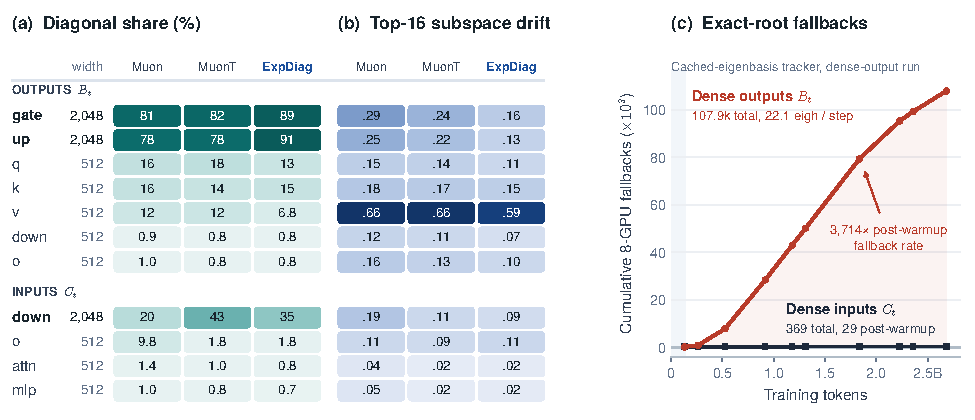
\includegraphics[width=\textwidth]{fig2_structural_audit.pdf}
 \caption{\textbf{Projection role separates moment geometry and drift across \mname{Muon}, \mname{MuonT}, and \mname{WT-MLP-Lag}.}
 \textbf{(a)} 32-layer median diagonal anisotropy share ($\mathrm{DiagAniso}$ in \cref{eq:diag_aniso}) at step 2,500 (130M); its complement is the off-diagonal share. Expanded SwiGLU outputs (\texttt{gate,up}) are predominantly diagonal across all three optimizers, whereas residual writers (\texttt{o,down}) carry less than 1\% of anisotropy on the diagonal.
 \textbf{(b)} 32-layer mean top-16 subspace drift from steps 2,250 to 2,500 (defined in \cref{eq:subspace_drift}; $0$ denotes identical subspaces and $1$ orthogonal subspaces).
 \textbf{(c)} Cumulative exact-eigendecomposition fallbacks across eight GPUs in the dense-output diagnostic run: dense outputs trigger 22.1 exact repairs per step versus 29 post-warmup fallbacks in total for dense inputs.}
 \label{fig:structural_audit}
\end{figure}

\begin{table}[tbp]\centering\footnotesize
\setlength{\tabcolsep}{5.8pt}
\caption{\textbf{Moment geometry and subspace drift by projection role at 130M.} Static columns report 32-layer medians on the Muon baseline trajectory at step 2,500 (matching \Cref{fig:overview}(a)). For diagonal anisotropy share (DA), parentheses give the range of these medians across Muon, MuonT, and Muon2-ExpDiag. $\rho_{\rm rms}$ is the RMS of off-diagonal uncentered correlations; root $R^2$ compares diagonal and dense inverse roots. Drift compares the subspaces at steps 2,250 and 2,500, averaged over 32 layers for each trajectory (ExpDiag denotes Muon2-ExpDiag). ExpDiag uses a resumed trajectory; uninterrupted-checkpoint comparisons are reported in \Cref{sec:output_drift}. Tinted expansion outputs account for 96.2\% of nominal dense output eigendecomposition work.}\label{tab:diagnosis_summary}
\begin{tabularx}{\textwidth}{@{}>{\raggedright\arraybackslash}Xrrrrrrr@{}}
\toprule
& & & \multicolumn{2}{c}{Diagonal fidelity} & \multicolumn{3}{c}{250-step $\mathrm{Drift}_{16}$} \\
\cmidrule(lr){4-5}\cmidrule(lr){6-8}
Moment & $d$ & $\rho_{\rm rms}$ & DA (\%, 3-traj) & Root $R^2$ (\%) & Muon & MuonT & ExpDiag \\
\midrule
\addlinespace[2pt]\multicolumn{8}{@{}l}{\textit{Input activation moments $C_t=\E[xx^{\Tr}]$ (4 per block)}}\\
attention & 512 & 0.147 & 1.4 (0.8--1.4) & 8.2 & 0.041 & 0.021 & 0.023 \\
o & 512 & 0.097 & 9.8 (1.8--9.8) & 30.1 & 0.107 & 0.094 & 0.108 \\
MLP & 512 & 0.141 & 1.0 (0.7--1.0) & 4.9 & 0.046 & 0.021 & 0.025 \\
down & 2,048 & 0.028 & 20.3 (20.3--43.4) & 91.3 & 0.186 & 0.106 & 0.087 \\
\addlinespace[5pt]\multicolumn{8}{@{}l}{\textit{Output cotangent moments $B_t=\E[\delta\delta^{\Tr}]$ (7 per block)}}\\
q & 512 & 0.061 & 16.4 (13.3--18.0) & 64.8 & 0.150 & 0.140 & 0.110 \\
k & 512 & 0.075 & 15.5 (14.4--15.5) & 77.6 & 0.178 & 0.165 & 0.147 \\
v & 512 & 0.060 & 11.5 (6.8--12.2) & 38.6 & 0.664 & 0.662 & 0.586 \\
\addlinespace[2.5pt]
o (res.) & 512 & 0.031 & 1.0 (0.8--1.0) & 3.6 & 0.164 & 0.134 & 0.103 \\
down (res.) & 512 & 0.032 & 0.9 (0.8--0.9) & 2.3 & 0.123 & 0.107 & 0.072 \\
\addlinespace[2.5pt]
\rowcolor{rowtint}[0pt][0pt]gate (exp.) & 2,048 & 0.005 & 80.6 (80.6--89.5) & 98.8 & 0.292 & 0.240 & 0.159 \\
\rowcolor{rowtint}[0pt][0pt]up (exp.) & 2,048 & 0.007 & 77.9 (77.9--90.8) & 98.2 & 0.251 & 0.215 & 0.130 \\
\bottomrule\end{tabularx}
\end{table}


\subsection{Dense correlations at hidden width; coordinate scaling at expansion width}
\label{sec:dichotomy}

\Cref{fig:structural_audit}(a) and \Cref{tab:diagnosis_summary} show a sharp separation by projection role. On the $\dff$-wide \texttt{gate} and \texttt{up} outputs, coordinate energy accounts for 78--91\% of total anisotropy across all three trajectories, off-diagonal correlations sit near $\rho_{\rm rms}=0.005\text{--}0.008$, and diagonal inverse roots capture 76--99\% of squared Frobenius distance to the dense inverse root. Structurally, these cotangents backpropagate through elementwise SwiGLU gates, multiplying the upstream gradient vector coordinatewise by token-dependent forward gating factors. The weak cross-channel correlations are consistent with this elementwise gating suppressing shared cross-channel output structure (though our empirical audit does not claim a general decorrelation theorem). Approximating these two moments with $L^{\mathsf{Diag}}$ and $\hat L^{\mathsf{Diag}}$ therefore preserves most of their conditioning while removing 96.2\% of nominal cubic output work in \cref{eq:cubic_share}.

The hidden-width residual writers \texttt{o} and \texttt{down} exhibit the opposite geometry. Unequal coordinate second moments account for only 0.8--1.0\% of their anisotropy, and diagonal inverse roots reduce squared error relative to identity by less than 4\% ($R^2=1.2\text{--}3.6\%$). Purely diagonal output preconditioning (\mname{OD-All}) thus acts nearly as identity on the projections writing back into the residual stream. The attention-internal outputs (\texttt{q,k,v}) fall between these regimes (7--18\% diagonal anisotropy; 20--79\% root $R^2$), carrying substantial off-diagonal structure at affordable width $\dm$ and motivating \mname{WT-MLP-Lag}'s retention of dense spectral roots on all five $\dm$-wide outputs.

Crucially, matrix width alone does not justify diagonalization on both sides. The equally wide $\dff=2{,}048$ \texttt{down} \emph{input} retains 57--80\% of its anisotropy off the diagonal ($\mathrm{DiagAniso}=20\text{--}43\%$, $\rho_{\rm rms}\approx 0.035$), as post-SwiGLU activations remain coupled through the shared $\dm$-dimensional token representation. This input--output asymmetry explains why \mname{WT-MLP-Lag} thresholds only the output side while keeping \texttt{in:down} dense—a choice confirmed empirically when symmetric $\dff$ diagonalization (\mname{WT-Sym-Lag}) sacrifices most of the loss gain in \Cref{sec:ablations}.

\subsection{Fast cotangent subspace drift requires asynchronous repairs}
\label{sec:drift_cost}

Even after removing $\dff\times\dff$ output eigendecompositions, the five $\dm$-wide output moments behave very differently over time from forward input moments (\Cref{fig:structural_audit}(b,c)). Along \mname{MuonT}, 250-step top-16 subspace drift is roughly $0.021$ on RMSNormed attention and MLP inputs, compared with $0.107\text{--}0.662$ across output cotangents. Consequently, a cached-eigenbasis root tracker that needs only 29 exact eigendecomposition fallbacks after warmup across all dense inputs triggers roughly 22 exact fallbacks \emph{per step} (107.9k cumulative across eight GPUs) when applied to dense outputs. (\Cref{sec:output_drift} extends this single-interval audit to uninterrupted checkpoints across full 130M and 520M training trajectories.)

Because cotangents arrive at the end of backpropagation, running distributed Gram reductions and frequent fallback eigensolves synchronously stalls every step boundary (\Cref{fig:method_pipeline}(b)). Pairing width thresholding with the $\tau=1$ asynchronous side-stream schedule in \Cref{sec:systems} addresses both halves of the cost bottleneck: mathematical approximation removes the $\dff^3$ solves, and one-step overlap hides most of the remaining $\dm^3$ repairs beneath the next forward and backward pass.
